\section{Brick Manufacturing Process}
% Information about the manufacturing process of bricks.

\subsection{Block Diagram}
% Description of the block diagram of the brick manufacturing process.
\begin{figure}[h]
  \centering
  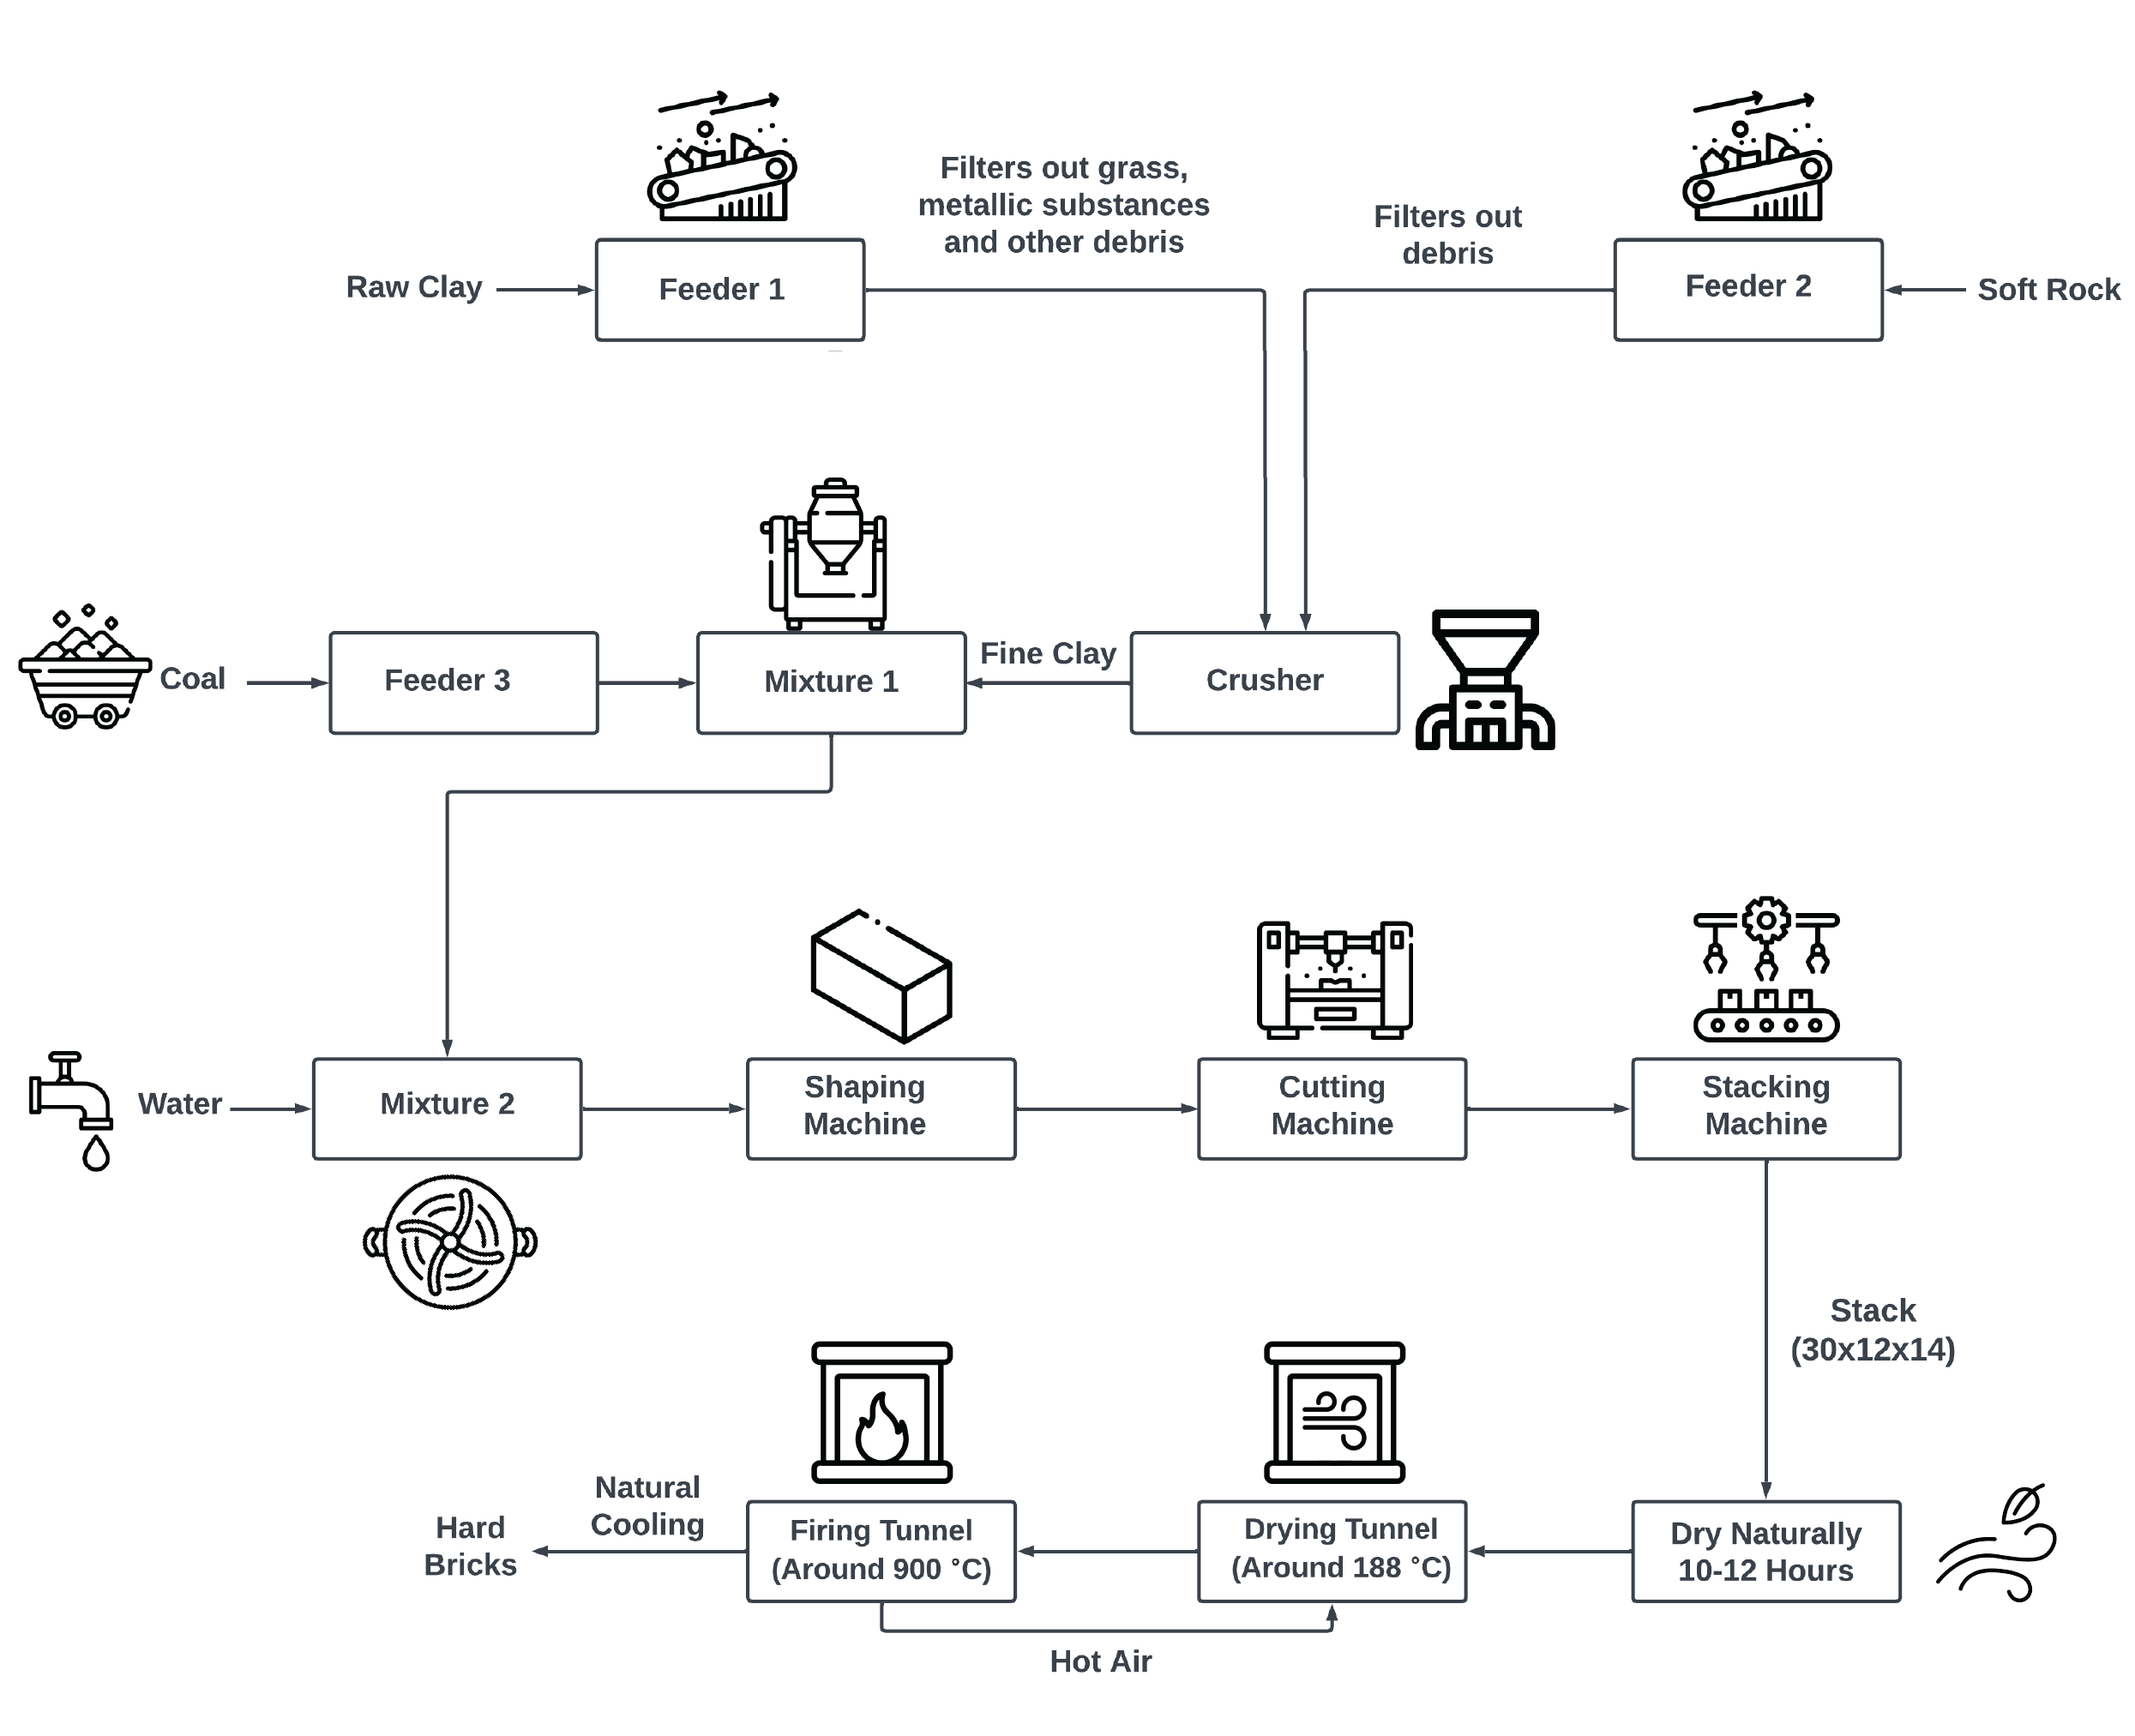
\includegraphics[width=1\textwidth]{img/block diagram.png}
  \caption{Block diagram for brick manufacture process}
\end{figure}

\subsection{Process Flow for Brick Manufacture}
Following are the basic steps of manufacturing bricks:\\
1.) Preparation of clay\\
2.) Cake making\\
3.) Drying\\
4.) Firing\\
5.) Cooling\\
\newpage
\large{\textbf{Clay processing}}\\
First large chunks of clay is strained through a giant strainer. The strainer helps to break down the chunks into smaller pieces. The smaller chunks are passed through a feeder. The clay is moved through a conveyor belt for filtering of grass and other unwanted debris. At different locations of conveyor belt, there are huge strong magnets placed above for filteing out metallic substances in the clay.\\
After the clay is roughly filtered, proper amount of soft rocks is added into the clay. The mixture is again passed through filtering process. Once the filtering process is good enough the mixture is hammered and mixed together to turn into finer mixture. Some amount of coal is added into the fine mixture and it is passed through another feeder into mixing machines. There are multiple mixing machines which mixes the clay properly. Into the machines, water is added into the clay to form dough-like mixture.